\section{AndroidDaily：面向日常生活 Agent 任务的动态基准}
\label{bmk_AndroidDaily}

\begin{figure}[t]
\centering
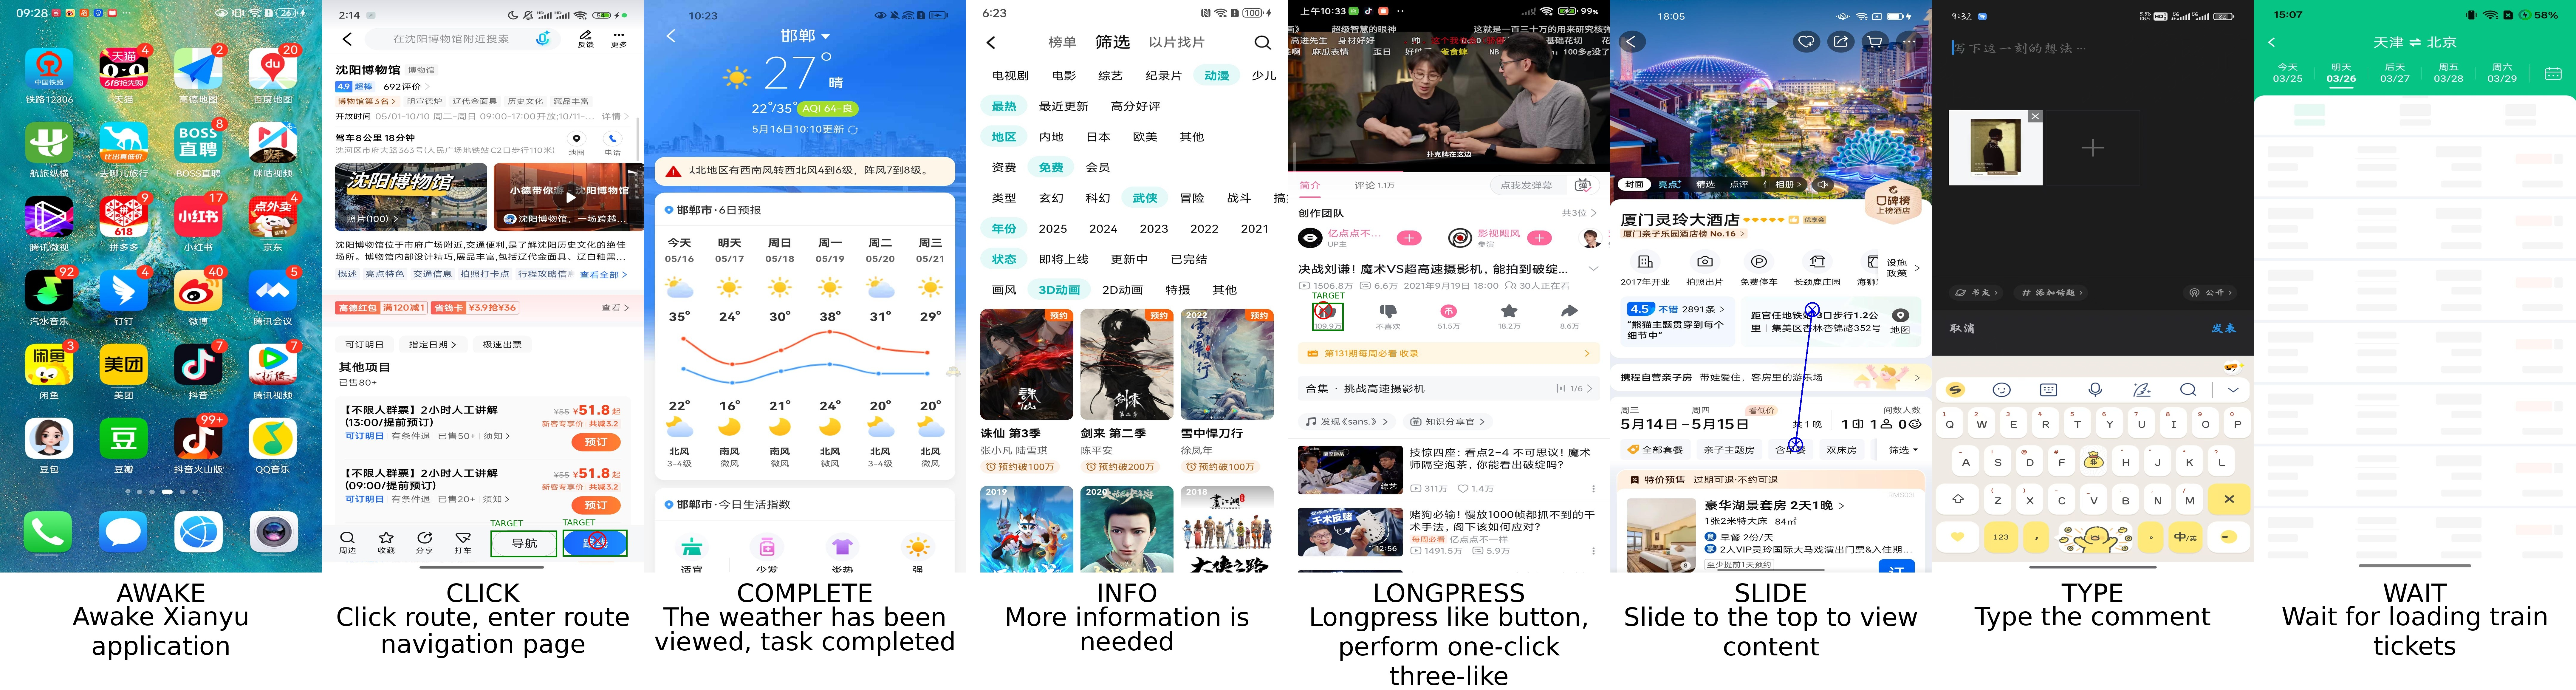
\includegraphics[width=\linewidth]{figs/android_daily_static.jpeg}
\caption{AndroidDaily 静态基准的动作分类。它覆盖 Android 自动化中的八类核心动作，并支持多解标注。}
\label{fig:android_daily_static}
\end{figure}

尽管 AndroidWorld 等基准已经推动了 Android GUI 智能体评测的发展，但现有基准与真实高频日常移动使用之间仍然存在明显差距。很多任务更偏向生产力或技术演示场景，而不一定是用户每天真正高频执行的事情。AndroidDaily 的设计目标正是填补这一空白。

与按应用目录选题不同，AndroidDaily 基于真实移动端使用频率与下载统计来选择任务场景。它重点覆盖出行、购物、社交媒体、娱乐和本地服务等高频应用场景，优先纳入外卖下单、打车、短视频浏览、移动支付等真实影响强、操作复杂度高、且与现实服务深度绑定的任务。

\begin{figure}[t]
\centering
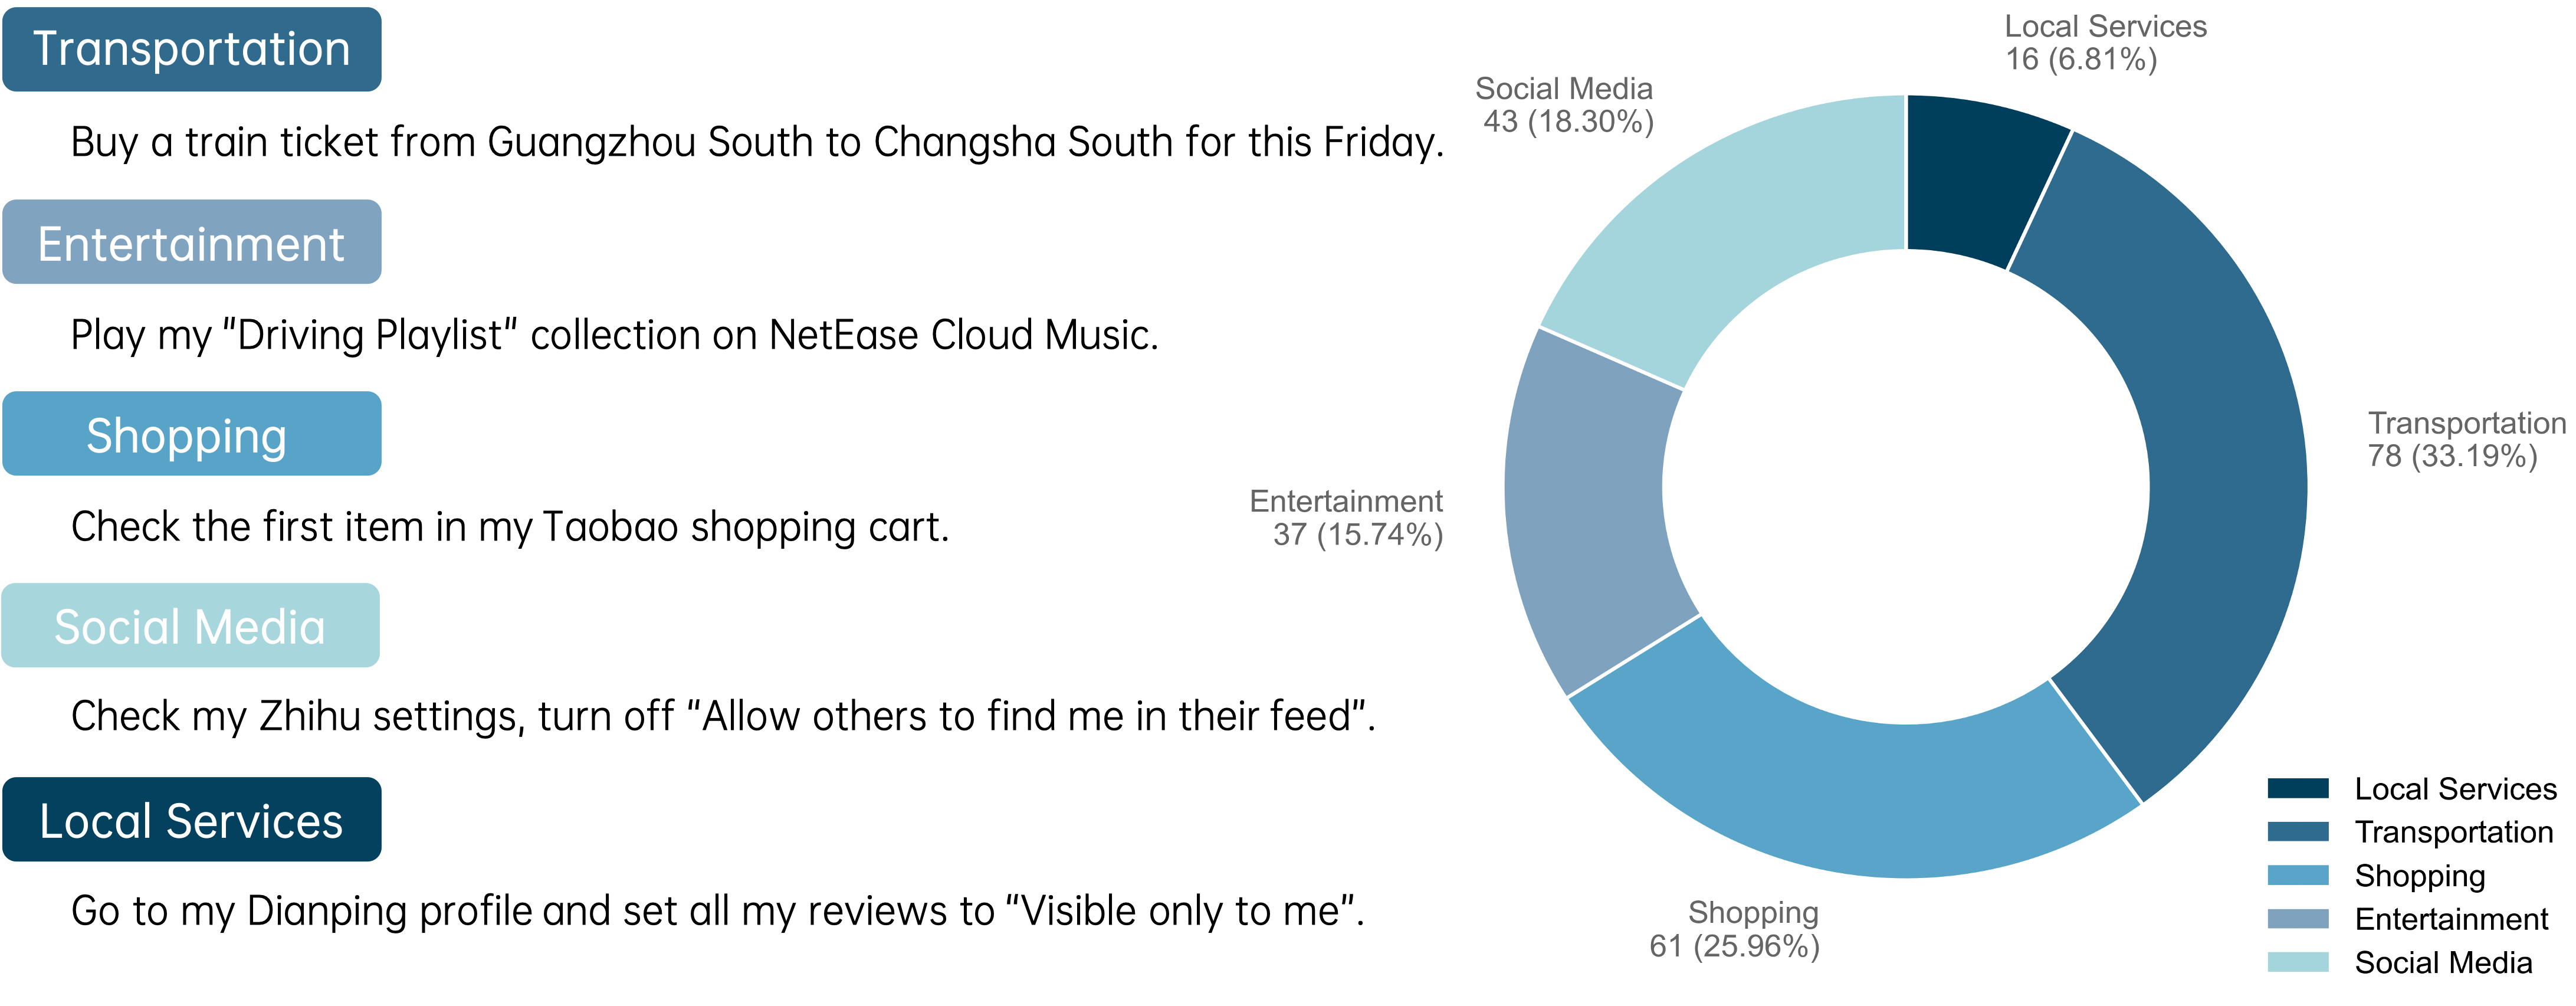
\includegraphics[width=\linewidth]{figs/scenario_distribution.png}
\caption{AndroidDaily 端到端任务的场景分布。该基准覆盖五类日常高频场景，并给出代表性任务示例。}
\label{fig:scenario_distribution}
\end{figure}

AndroidDaily 采用双层评测设计，以平衡评测效率与真实性。

\paragraph{静态基准（3146 个动作）。}
静态基准提供任务描述与逐步截图，要求模型预测当前界面上的下一步动作。它覆盖 AWAKE、CLICK、COMPLETE、INFO、LONGPRESS、SLIDE、TYPE 和 WAIT 八类动作。每个动作都带有精确参数，且显式支持多解 ground truth，例如同一个目标可能可通过多个 UI 区域完成。该设置适合高效迭代模型，因为不需要复杂的在线环境。

\paragraph{端到端基准（235 个任务）。}
端到端基准要求智能体在真实应用环境中完成整项任务，并通过 LLM-based judge 判定是否成功。这种设置工程成本更高，但更接近真实世界使用。任务主要分布在五类日常场景中：\textit{Transportation}、\textit{Shopping}、\textit{Social Media}、\textit{Entertainment} 与 \textit{Local Services}。

除场景类别之外，AndroidDaily 还从多个维度标注任务属性，包括认知操作类型（检索、筛选、分析等）、结构复杂度（原子任务、组合任务、带条件/循环任务）以及指令歧义等级。这样的多维组织方式有助于精确分析模型的强项与失败模式，也让这个基准比传统“纯动作匹配”式评测更具诊断价值。
